\documentclass[11pt,letterpaper]{article}
\usepackage[T1]{fontenc}
\usepackage{lmodern}
\usepackage[margin=0.85in]{geometry}
\usepackage{booktabs,array,graphicx,placeins,float}
\usepackage[hidelinks]{hyperref}
\hypersetup{pdftitle={Copilot Review Verdicts, Approval Records, and Pull Request Merges},
pdfauthor={Ogtay Hasanov}}
\setlength{\parindent}{0pt}
\setlength{\parskip}{4pt plus 1pt}
\setlength{\emergencystretch}{2em}
\widowpenalty=10000
\clubpenalty=10000
\newcommand{\FrameCount}{79,296}
\newcommand{\CompleteLists}{76,113}
\newcommand{\UnavailableLists}{3,181}
\newcommand{\ErrorLists}{2}
\newcommand{\MissingStateLists}{23}
\newcommand{\LinkedStateLists}{76,090}
\newcommand{\OutcomePRs}{69,801}
\newcommand{\OutcomeMerged}{59,759}
\newcommand{\OverallMatches}{33,977}
\newcommand{\OverallComparable}{59,647}
\newcommand{\UnknownComparedSHAs}{112}
\newcommand{\ChangesMatches}{6,437}
\newcommand{\ChangesComparable}{22,590}
\newcommand{\ChangesMismatches}{16,153}
\newcommand{\PostMergeCount}{5,951}
\newcommand{\PostMergeDenominator}{65,710}
\newcommand{\NoCurrentMergedReview}{41}
\newcommand{\FormalPRs}{429}
\newcommand{\FormalMerged}{418}
\newcommand{\FormalClosed}{4}
\newcommand{\FormalOpen}{7}
\newcommand{\FormalNoUser}{389}
\newcommand{\FormalBotAuthor}{43}
\newcommand{\FormalMatches}{410}
\newcommand{\FormalComparable}{418}
\newcommand{\FormalMismatches}{8}
\newcommand{\AuditSample}{2,000}
\newcommand{\AuditAccessible}{1,923}
\newcommand{\AuditInaccessible}{77}
\newcommand{\AuditMissingState}{2}
\newcommand{\AuditLinked}{1,921}
\newcommand{\AuditReviewCount}{7,355}
\newcommand{\AuditMissingReviews}{5,056}
\newcommand{\AuditMissingPRs}{870}
\newcommand{\AuditGroupChanges}{348}
\newcommand{\ProbeMissingTested}{50}
\newcommand{\ProbeMissingFound}{0}
\newcommand{\ProbeControlsTested}{10}
\newcommand{\ProbeControlsFound}{10}
\newcommand{\ReadyMatchRate}{78.0\%}
\newcommand{\CoverageRate}{96.0\%}
\newcommand{\ReadyMergeRate}{89.7\%}
\newcommand{\ChangesMergeRate}{81.9\%}
\newcommand{\ChangesMatchRate}{28.5\%}
\newcommand{\ChangesMismatchRate}{71.5\%}
\newcommand{\OverallMatchRate}{57.0\%}
\newcommand{\PostMergeRate}{9.1\%}
\newcommand{\FormalNoUserRate}{93.1\%}
\newcommand{\FormalMatchRate}{98.1\%}
\newcommand{\AuditMissingReviewRate}{68.7\%}
\newcommand{\AuditMissingPRRate}{45.2\%}
\newcommand{\AuditGroupChangeRate}{18.1\%}
\newcommand{\MergeGapPP}{7.8}
\newcommand{\AuditMissingPRLowCI}{43.0}
\newcommand{\AuditMissingPRHighCI}{47.5}
\newcommand{\AuditGroupChangeLowCI}{16.5}
\newcommand{\AuditGroupChangeHighCI}{19.9}
\newcommand{\RepositoryLink}{\par Replication repository: \url{https://github.com/ogtayhasanov/copilot-review-study}.}
\newcommand{\FormalBaselineCount}{389}
\newcommand{\FormalBaselinePRs}{418}
\newcommand{\FormalBaselineRate}{93.1\%}
\newcommand{\TextBaselineCount}{40,702}
\newcommand{\TextBaselinePRs}{59,759}
\newcommand{\TextBaselineRate}{68.1\%}
\newcommand{\NonformalBaselineCount}{40,313}
\newcommand{\NonformalBaselinePRs}{59,341}
\newcommand{\NonformalBaselineRate}{67.9\%}
\newcommand{\SharedBaselineCount}{1,114}
\newcommand{\SharedBaselinePRs}{1,193}
\newcommand{\SharedBaselineRate}{93.4\%}
\newcommand{\PeriodBaselineCount}{1,100}
\newcommand{\PeriodBaselinePRs}{1,179}
\newcommand{\PeriodBaselineRate}{93.3\%}
\newcommand{\FormalRepoCount}{137}
\newcommand{\FormalRepoTopOnePRs}{104}
\newcommand{\FormalRepoTopOneRate}{24.2\%}
\newcommand{\FormalRepoTopFivePRs}{167}
\newcommand{\FormalRepoTopFiveRate}{38.9\%}
\newcommand{\FormalRepoTopTenPRs}{198}
\newcommand{\FormalRepoTopTenRate}{46.2\%}
\newcommand{\MergedFormalRepoCount}{133}
\newcommand{\MergedFormalRepoTopOnePRs}{104}
\newcommand{\MergedFormalRepoTopOneRate}{24.9\%}
\newcommand{\MergedFormalRepoTopFivePRs}{166}
\newcommand{\MergedFormalRepoTopFiveRate}{39.7\%}
\newcommand{\MergedFormalRepoTopTenPRs}{197}
\newcommand{\MergedFormalRepoTopTenRate}{47.1\%}
\newcommand{\FirstFormalDate}{3 September 2026}

\title{Copilot Review Verdicts, Approval Records, and Pull Request Merges}
\author{Ogtay Hasanov}
\date{14 November 2026}
\begin{document}
\maketitle

\begin{abstract}
Since September 2026, GitHub Copilot can end a code review with a verdict:
recommend approval, recommend changes, or take a closer look. We examine
what happens to pull requests (PRs) after each verdict. We obtained
complete review lists for \CompleteLists{} public PRs. The verdict
analysis includes \OutcomePRs{} of them. After a changes verdict, the saved PR commit matched the reviewed
commit in \ChangesMatchRate{} of merged PRs with usable commit records.
After an approval verdict, that share was \ReadyMatchRate{}. PRs merged less
often after a changes verdict (\ChangesMergeRate{}). After an approval
verdict, the merge rate was \ReadyMergeRate{}. Copilot also issued
formal approvals, but these were rare (\FormalPRs{} PRs). They occurred
in repositories where user-account approvals were already uncommon.
In a random validation sample, our GH Archive export lacked
\AuditMissingReviewRate{} of qualifying Copilot review records. Adding
missing reviews changed the assigned verdict for \AuditGroupChangeRate{}
of sampled PRs with saved outcomes. Our results describe review records
and commit identity. They do not measure code quality.

\end{abstract}

\section{Introduction}

Code review helps developers decide what to change and when a pull
request is ready to merge. Copilot adds an overall verdict to this
process: recommend approval, recommend changes, or take a closer look.
GitHub introduced these verdicts in September 2026
\cite{github_assessments}. Copilot can also issue a formal approval that
counts toward a repository's approval rules \cite{github_approvals}.
The text verdict and formal approval are separate records.

We examine how these records relate to what happens to a PR. A changes
verdict may be followed by revisions, closure, or a merge. An approval
may arrive before the merge or after it. We link Copilot's review
records to saved PR outcomes and compare the reviewed commit with the
saved commit. Section~3 defines these records and the selection rules.

After a changes verdict, the saved PR commit matched the reviewed
commit in \ChangesMatchRate{} of merged PRs with usable commit records.
After an approval verdict, that share was \ReadyMatchRate{}. Most PRs in both groups merged.
We report their merge rates alongside the commit comparisons and check
how the rates change when open PRs are excluded.

Formal approvals need repository context. Most merged PRs with a formal
Copilot approval had no user-account approval recorded by merge
(\FormalNoUserRate{}). The same was true for comparison PRs in those
repositories (\SharedBaselineRate{}). We therefore report the formal
approval result together with its comparison groups and repository
concentration.

The review source also changes the result. In a random validation
sample, adding reviews missing from our archive export changed the
assigned verdict on \AuditGroupChangeRate{} of PRs with saved outcomes.
We use API review histories for the outcome analysis and report the
archive check so that the effect of missing reviews is visible.

\section{Related work}

Sun et al.\ study whether comments from AI review tools run through GitHub
Actions are followed by code changes \cite{sun2025}. Cynthia et al.\
examine developer responses to review comments from coding agents
\cite{cynthia2026}. Selvanayagam and Ghaleb study PRs authored and reviewed
by AI agents using agent-attributed GitHub events
\cite{selvanayagam2026}. These studies focus on comments, their resolution,
or the agents on each side of a review. Our unit is Copilot's overall
verdict of a PR, linked to its review history, saved commit, and outcome.

Manji examines the provenance of formal approvals in one company's merge
workflow \cite{manji2026}. That work also shows why an account recorded as
a user can carry automated activity. We use GitHub's account types as
recorded metadata. Formal approvals and verdict headings are separate
properties in our analysis.

\section{Data and measures}

\subsection{Frozen archive export and outcomes}

We queried public \texttt{PullRequestReviewEvent} records from GH Archive
for 1 September through 9 November 2026, inclusive in UTC
\cite{gharchive}. We retained creation and update actions and selected
one version per repository and review ID, preferring a creation event.
We identified Copilot using the lowercased review-user login, with the
event actor as a fallback. Accepted logins were \texttt{copilot},
\texttt{copilot-pull-request-reviewer}, and
\texttt{copilot-pull-request-reviewer[bot]}.

The extractor recognized the headings \emph{Approval recommended},
\emph{Changes recommended}, and \emph{Needs a closer look}, including their
status emoji. The export contained 95,414 classified reviews on \FrameCount{}
distinct PRs. A separate export confirmed that every selected timestamp
matched GitHub's native review submission time.

We linked 76,217 input PRs to usable GitHub GraphQL snapshots
\cite{github_graphql}. These recorded PR state, opening and terminal
times, PR commit identifier, and account types. The initial collection supplied
35,747 snapshots, and recovery completed on 10 November 2026 added
40,470. We retain these frozen outcomes when analyzing the review lists
retrieved later.

\subsection{Random validation and raw-archive probe}

We drew a simple random sample of \AuditSample{} distinct PRs from the \FrameCount{}-PR
roster, using seed 20261112. We fetched their review lists through the
GitHub REST API and followed pagination \cite{github_reviews}. We resolved
renamed repositories when possible and obtained complete lists for
\AuditAccessible{} PRs. The other 77 were inaccessible. Two accessible PRs lacked
a usable frozen outcome, leaving \AuditLinked{} for verdict-group comparisons.

The reconciliation uses the same reviewer identities, verdict
headings, and UTC submission window as the frozen export. The API lists
supplied \AuditReviewCount{} qualifying reviews. We matched records by PR and native
review ID. For each PR, we added missing API reviews to the frozen list,
retained its existing records, and recomputed the selected verdict
and all-after-merge status. We also computed the selected group directly
from the API lists. The group-change count was the same under both
approaches. Two archived IDs were absent from the API lists, and ten
shared records differed in their associated commit identifier. No shared qualifying
review changed class. Audit proportion intervals use the Wilson method.

We then sampled 50 of the 5,056 missing review IDs, using seed 20261112.
We selected ten known-present IDs as positive controls, using seed
20261113. One BigQuery query searched the raw
\texttt{PullRequestReviewEvent} tables for the same archive window by
review ID, with no reviewer or heading filter. It returned one diagnostic
row for each of the 60 targets, including explicit zero counts.
The checked missing reviews spanned 43 repositories. This probe tests
raw presence for those IDs in that window. It does not identify the
upstream reason for an absent event.

\subsection{Review lists for the full roster}

After validation, we attempted to fetch review lists for every PR in the
original roster. We reused the \AuditAccessible{} complete validation lists and
collected the remainder through the REST and GraphQL APIs on
12--13 November 2026. The GraphQL collector requests multiple PRs in
a batch and follows every review cursor. Before switching transports,
a check compared four reviews on one PR across both APIs. Native review
IDs, submission times, reviewed commit identifiers, states, and verdict fields matched.

The completed pass obtained complete review lists for \CompleteLists{} PRs
(\CoverageRate{} of the roster). Another \UnavailableLists{} PRs were unavailable, and \ErrorLists{} had
collection errors. Of the complete lists, \MissingStateLists{} lacked a usable frozen
state. The outcome analysis therefore starts from \LinkedStateLists{} PRs with both
a complete review list and a usable state. These counts describe
coverage of the input frame; PRs absent from that frame are outside
the study.

\subsection{Selecting verdicts and computing rates}

We call a recognized overall text recommendation a \emph{verdict}.
The \emph{reviewed commit} is the commit identified by its review.
The \emph{saved commit} is the PR commit recorded in the frozen outcome
snapshot. We compare their Git commit identifiers to determine whether
they identify the same commit.

A verdict qualifies for outcome grouping if it has a recognized
heading and a native submission time in the study window, at or after
PR opening and, for a terminal PR, at or before merge or closure.
We sort the reviews by submission time and select the last qualifying
verdict. Tied timestamps with conflicting classes are excluded.
For an open PR, selection uses the last qualifying verdict in the
study window. This yielded \OutcomePRs{} PRs.

A group's merge rate divides the number of its PRs recorded as merged
by every PR in that group, including open and closed PRs. The commit-match
rate among merges divides equal reviewed and saved commit identifiers by the merged
PRs with comparable commit identifiers. We exclude missing or ambiguous compared commit identifiers
from this second denominator. There were \UnknownComparedSHAs{} such records among the
\OutcomeMerged{} merged PRs in the outcome table.

The timing analysis includes all \PostMergeDenominator{} linked merged PRs with a current
qualifying review, including PRs whose verdicts fall outside the
pre-merge outcome grouping. A PR is classified as assessed only after
merge when every qualifying review has a submission time strictly later
than the recorded merge time. Another \NoCurrentMergedReview{} linked merged PRs had no current
qualifying review and remain unclassified for this timing rate.

A formal approval state is distinct from a verdict heading. A later
formal approval without a recognized heading does not supersede the last
qualifying verdict used in Table~\ref{tab:outcomes}. In the
validation sample, none of the \SampleFormalReviews{} qualifying Copilot
approval reviews carried a recognized verdict heading. Thus a PR's
selected verdict can precede a later formal approval. At most
\FormalMerged{} merged text-cohort PRs (\FormalShareOfMergedText{}) have
a qualifying formal Copilot approval. Even if all of them were
merges with different commits in the changes group, excluding them would raise
that group's matching-commit share only from \ChangesMatchRate{} to
\ChangesFormalBoundRate{}. This is a conservative upper bound, not an
observed reclassification of all formal-approval PRs.

A formal approval is identified independently of the text heading,
using a Copilot review whose current API state is \texttt{APPROVED},
submitted in the study window and within the observed PR lifetime.
For a merged PR, we consider only approvals submitted by merge. The
formal-approval commit comparison uses the last such approval, excluding
ambiguous tied commit identifiers. A user-account approval is a returned, non-Copilot
\texttt{APPROVED} review by an account GitHub classifies as \texttt{User},
submitted at or after PR opening and by merge.

\subsection{Approval-record baselines and repository concentration}

We applied the same user-account approval definition to every merged PR
in the verdict cohort. User approvals need not fall within the
Copilot verdict study window; they must be submitted within the PR
lifetime and by the frozen merge time. All \FormalMerged{} merged
formal-approval PRs also belong to the verdict cohort. We report
the full baseline and a baseline excluding these formal-approval PRs.

For repository context, we restricted the nonformal comparison PRs to
repositories represented by the full \FormalPRs{}-PR formal-approval
cohort. A further descriptive restriction retained PRs merged on or after
the earliest qualifying formal approval observed in that cohort
(\FirstFormalDate{}). This is a lower time cutoff, rather than a matched
follow-up design. These comparisons remain conditional on the
Copilot-reviewed input frame and do not adjust for repository approval
rules, PR composition, or author behavior.

We counted distinct repositories and the shares contributed by the
largest repositories for both the full formal-approval cohort and its
merged subset. Repository identity uses the saved canonical repository
name when available, otherwise the original roster name. This combines
saved aliases for renamed repositories.

\subsection{Checking the saved commit}

We drew a separate random sample of 20 merged PRs from the linked frozen
roster, using seed 20261113. For each, we compared the saved commit with
the current PR commit and the last commit in the complete PR commit list
\cite{github_commits}. All 20 saved commits matched both API values.
Five PRs had a two-parent merge commit, and the saved commit matched its
second parent in all five. This directly verifies the PR commit at merge for
those five cases. Squash and rebase merges lack this second-parent check.
We use \emph{PR commit at merge} for the five verified cases and \emph{saved commit}
for the combined tables.

\section{Results}

\subsection{Merges after changes verdicts}

After a changes verdict, the saved PR commit matched the reviewed
commit in \ChangesMatchRate{} of merged PRs with usable commit records.
After an approval verdict, that share was \ReadyMatchRate{}.
Most merged PRs in the changes group had a different saved commit
(\ChangesMismatchRate{}). Across all verdict groups, the
reviewed and saved commits matched in \OverallMatchRate{} of comparable
merges. Table~\ref{tab:outcomes} gives the counts and denominators.

Most PRs merged in both the approval and changes groups. Merges were
more common after approval verdicts (\ReadyMergeRate{}) than after
changes verdicts (\ChangesMergeRate{}). The gap was \MergeGapPP{}
percentage points.

The gap narrowed when open PRs were excluded (\TerminalMergeGapPP{}
percentage points). Among PRs recorded as merged or closed, merge rates
were \ReadyTerminalMergeRate{} after approval verdicts
(\ReadyMerged{}/\ReadyTerminalPRs{}) and \ChangesTerminalMergeRate{}
after changes verdicts (\ChangesMerged{}/\ChangesTerminalPRs{}).
Open PRs were more common in the changes group (\ChangesOpenRate{})
than in the approval group (\ReadyOpenRate{}).

\begin{table}[H]
\centering
\caption{Outcomes by last qualifying text assessment. Merge rates use every PR in the group. Head-match rates use comparable merged PRs.}
\label{tab:outcomes}
\small
\begin{tabular}{@{}lrrr@{}}
\toprule
Assessment & PRs & Merged & Matching heads among merges \\
\midrule
Approval recommended & 23,967 & 21,503 (89.7\%) & 16,755/21,473 (78.0\%) \\
Changes recommended & 27,648 & 22,648 (81.9\%) & 6,437/22,590 (28.5\%) \\
Needs a closer look & 18,186 & 15,608 (85.8\%) & 10,785/15,584 (69.2\%) \\
All & 69,801 & 59,759 (85.6\%) & 33,977/59,647 (57.0\%) \\
\bottomrule
\end{tabular}
\end{table}


\begin{figure}[H]
\centering
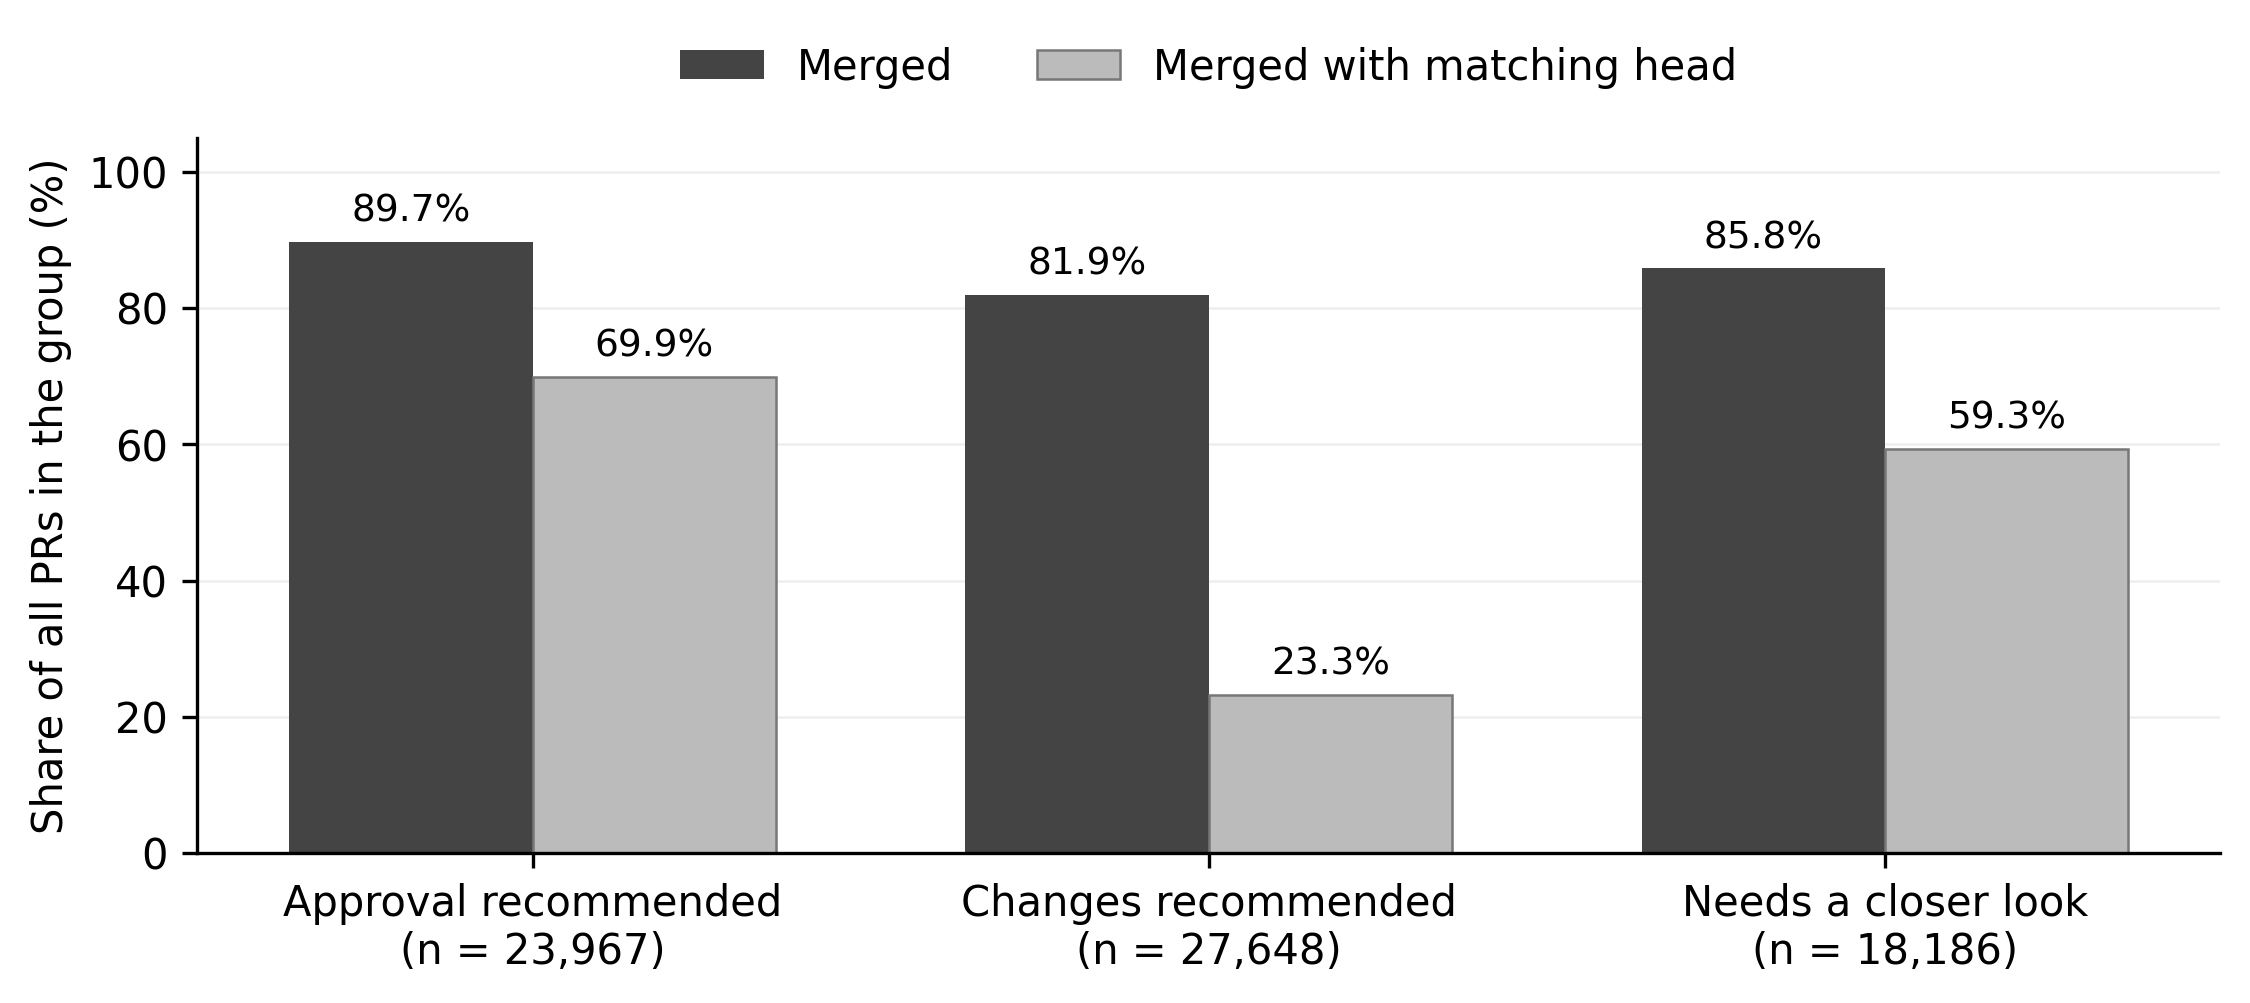
\includegraphics[width=0.96\linewidth]{generated/merge_outcomes.png}
\caption{Both bars count all PRs in each verdict group. The lighter bar
counts PRs that merged and had matching reviewed and saved commits.
PRs with missing or ambiguous commit records stay in the group total
but do not contribute to the lighter bar.}
\label{fig:outcomes}
\end{figure}

\subsection{Formal approvals and user-account approvals}

Most merged PRs with a formal Copilot approval had no current
user-account approval recorded by merge (\FormalNoUserRate{}).
Table~\ref{tab:formal} reports the merged cases. Formal approvals were
rare: the full group contained \FormalPRs{} PRs. Of these,
\FormalMerged{} merged, \FormalClosed{} closed, and \FormalOpen{}
remained open.

\begin{table}[H]
\centering
\caption{Formal Copilot approvals. The merged rate uses all qualifying formal-approval PRs. The remaining rows describe the merged subset.}
\label{tab:formal}
\small
\begin{tabular}{@{}p{0.60\linewidth}rr@{}}
\toprule
Measure & Count & Share \\
\midrule
Recorded as merged & 418/429 & 97.4\% \\
Merged with no current user-account approval record dated by merge & 389/418 & 93.1\% \\
Merged PR authored by an account classified as a bot & 43/418 & 10.3\% \\
Last formal-approval SHA matched the saved head & 410/418 & 98.1\% \\
\bottomrule
\end{tabular}
\end{table}


The last formally approved commit usually matched the saved commit
(\FormalMatchRate{}). The commits matched in \FormalMatches{} of
\FormalComparable{} merged cases and differed in \FormalMismatches{}.

\subsection{Repository context}

The high share of PRs without a user-account approval also appeared in
the comparison PRs from the same repositories. The share was
\TextBaselineRate{} across all merged PRs with a usable verdict.
Excluding PRs with a formal Copilot approval gave
\NonformalBaselineRate{}. In the repositories represented in the formal
approval group, the comparison share was \SharedBaselineRate{}.
Applying the additional time cutoff gave \PeriodBaselineRate{}.
Table~\ref{tab:approval-context} gives each comparison and its denominator.

\begin{table}[H]
\centering
\caption{Current user-account approval records among merged PRs. Each row counts PRs without a qualifying user-account approval by merge. Repository-restricted rows exclude formal Copilot approvals and use repositories represented in the full formal-approval cohort.}
\label{tab:approval-context}
\small
\begin{tabular}{@{}p{0.60\linewidth}rr@{}}
\toprule
Merged PR group & Count & Share \\
\midrule
Formal Copilot approvals & 389/418 & 93.1\% \\
All merged text-assessment PRs & 40,702/59,759 & 68.1\% \\
Text-assessment PRs without formal Copilot approval & 40,313/59,341 & 67.9\% \\
Nonformal comparison PRs in formal-cohort repositories & 1,114/1,193 & 93.4\% \\
Same repositories, merged on/after first formal approval & 1,100/1,179 & 93.3\% \\
\bottomrule
\end{tabular}
\end{table}


The formal approval group's \FormalNoUserRate{} share was higher than
the overall baseline but close to both comparisons within those
repositories. A high rate of absent user-account approval records was
therefore not distinctive to the formal approval group in this setting.

Formal approvals were spread across \FormalRepoCount{} repositories,
but their contributions were uneven. The largest contributed
\FormalRepoTopOnePRs{} PRs (\FormalRepoTopOneRate{}), and the top five
contributed \FormalRepoTopFivePRs{} (\FormalRepoTopFiveRate{}).
The merged cases covered \MergedFormalRepoCount{} repositories.
Their largest contributor supplied \MergedFormalRepoTopOnePRs{}
(\MergedFormalRepoTopOneRate{}), and their top five supplied
\MergedFormalRepoTopFivePRs{} (\MergedFormalRepoTopFiveRate{}).

\subsection{Verdicts after merge}

Some PRs received all their qualifying verdicts after they had already
merged (\PostMergeRate{}). This occurred on \PostMergeCount{} of
\PostMergeDenominator{} merged PRs with a current qualifying verdict.
Another \NoCurrentMergedReview{} merged PRs had no current qualifying
verdict and were excluded from this rate.

\subsection{Missing reviews in the archive export}

The archive export missed reviews on many PRs in the validation sample
(\AuditMissingPRRate{}). The confidence interval ran from
\AuditMissingPRLowCI{} to \AuditMissingPRHighCI{}. At review level,
most qualifying API review records were absent from the export
(\AuditMissingReviewRate{}). Adding the missing reviews changed the
assigned verdict for \AuditGroupChangeRate{} of sampled PRs with saved
outcomes. The confidence interval ran from \AuditGroupChangeLowCI{}
to \AuditGroupChangeHighCI{}. Both intervals use a 95\% confidence level.
Table~\ref{tab:audit} gives the counts and denominators.

\begin{table}[H]
\centering
\caption{Validation of the frozen export. Review-level and PR-level denominators are stated separately.}
\label{tab:audit}
\small
\begin{tabular}{@{}p{0.60\linewidth}rr@{}}
\toprule
Measure & Count & Share \\
\midrule
Complete review lists in the random validation sample & 1,923/2,000 & 96.2\% \\
PRs with a qualifying API review absent from the export & 870/1,923 & 45.2\% \\
Qualifying API reviews absent from the export & 5,056/7,355 & 68.7\% \\
Selected group changed after adding missing reviews & 348/1,921 & 18.1\% \\
All-after-merge status changed after adding missing reviews & 12/1,642 & 0.7\% \\
\bottomrule
\end{tabular}
\end{table}


The raw-archive check also found none of the \ProbeMissingTested{}
sampled missing review IDs. All \ProbeControlsTested{} positive controls
were found. The checked records were therefore absent from the scanned
archive tables before our reviewer and verdict-heading filters were
applied.

\section{Interpretation and limits}

The results describe review records, PR outcomes, and commit identity.
They do not measure code quality or verdict correctness. A merge after a
changes verdict can follow a repair, an unrelated edit, or a decision to
proceed. The records do not establish which findings were addressed or
whether Copilot caused an edit.

User-account approvals are account records. An account classified as
\texttt{User} can run automated activity, and a prior approval can later
be dismissed. An absent current approval record does not establish
whether a person inspected the PR or whether branch rules required
human approval.

The comparisons within repositories are unadjusted descriptions.
Similar aggregate rates do not establish equivalence between groups or
identify Copilot's effect on approval behavior. The concentration of
formal approvals also limits generalization across repositories.

The input frame contains public PRs with at least one verdict
captured by the original extraction. PRs entirely absent from that frame
are outside the study. The full-roster collection obtained complete
lists for \CoverageRate{} of input PRs. The \UnavailableLists{} unavailable PRs, \ErrorLists{} collection
errors, and \MissingStateLists{} complete lists without usable frozen outcomes can differ
from the included cases. Availability is not assumed random.

The archive probe establishes absence of the checked IDs from the
scanned \texttt{PullRequestReviewEvent} tables. It does not determine why
they were absent. We did not verify historical public visibility for
every repository or test every missing ID against all possible archive
dates. Capture rates for other reviewer types were not measured in this
audit. The validation sample's missing-review rate therefore remains
a measurement of the frozen export, with a targeted raw-archive check.

The API histories reflect records available when fetched on
12--13 November 2026. Text and review states can change, and deleted
records can be unavailable. Submission time dates the review record;
a verdict heading can have been added later. Pagination is not an
atomic snapshot of a changing PR.

The outcomes remain frozen at their earlier collection times. PRs
opened on different dates have different amounts of follow-up, and open
PRs can merge later. Merge-rate gaps are observed associations; this
analysis does not adjust them for PR size, repository practices,
author type, or elapsed time.

The saved commit is a snapshot measurement. It is directly verified as
the PR commit at merge for the five second-parent checks. Current API
agreement alone does not supply that historical verification across
the full group. Matching identifiers establish the same commit, but
intermediate commits may have been pushed and later removed. Different
identifiers can represent equivalent code after a rebase. A different
reviewed commit may also remain an ancestor of the saved commit.

\section{Conclusion}

The reviewed and saved commits matched less often after changes verdicts.
After a changes verdict, the saved PR commit matched the reviewed commit
in \ChangesMatchRate{} of merged PRs with usable commit records. After an
approval verdict, that share was \ReadyMatchRate{}. Most PRs in both
groups merged, with a gap of \MergeGapPP{} percentage points between
their merge rates.

Formal approvals need repository context. Most merged PRs with a formal
Copilot approval had no current user-account approval recorded by merge
(\FormalNoUserRate{}). The comparison share in those repositories was
\SharedBaselineRate{}. Formal approvals were spread across many
repositories, but the top five contributed \FormalRepoTopFiveRate{}
of the cases.

Some PRs received all their qualifying verdicts after merge
(\PostMergeRate{}). Adding reviews missing from the archive export
changed the assigned verdict for \AuditGroupChangeRate{} of sampled PRs
with saved outcomes. Review timing, repository context, and complete
histories are central to interpreting these outcomes.

\section{Reproducibility and AI assistance}

Replication materials include frozen inputs and outcomes, selected PR-level
verdict results, validation samples, collection and analysis
scripts, and the approval-context audit. The build regenerates
Tables~\ref{tab:outcomes}--\ref{tab:audit}, Figure~\ref{fig:outcomes}, and
percentages from saved machine-readable results. The raw-archive query
and its result are included.

The full native-review \texttt{reviews.sqlite} checkpoint is retained
locally and is not bundled. Independently recounting formal approvals
and approval-record baselines requires that checkpoint. The context audit
verifies the reconstructed text cohort and original formal counts against
the saved analysis before computing additional aggregates.
\RepositoryLink{}

ChatGPT assisted with script development, analysis checks, and drafting.


\begin{thebibliography}{99}
\small
\setlength{\itemsep}{2pt}
\bibitem{github_assessments}
GitHub. \href{https://github.blog/changelog/2026-09-01-copilot-code-review-can-now-approve-pull-requests/}
{Copilot code review can now approve pull requests}. GitHub Changelog,
1 September 2026.
\bibitem{github_approvals}
GitHub. \href{https://github.blog/changelog/2026-10-28-copilot-code-review-merge-with-confidence-with-max-and-approvals/}
{Copilot code review: Merge with confidence with Max and approvals}.
GitHub Changelog, 28 October 2026.
\bibitem{sun2025}
Kexin Sun, Hongyu Kuang, Sebastian Baltes, Xin Zhou, He Zhang, Xiaoxing Ma,
Guoping Rong, Dong Shao, and Christoph Treude.
\href{https://arxiv.org/abs/2508.18771}{Does AI Code Review Lead to Code Changes?
A Case Study of GitHub Actions}. arXiv:2508.18771, 2025.
\bibitem{cynthia2026}
Shamse Tasnim Cynthia, Ratnadira Widyasari, Banani Roy, Ting Zhang, and David Lo.
\href{https://arxiv.org/abs/2607.21997}{\textquotedblleft Go Home Copilot,
You're Drunk\textquotedblright: Understanding Developer Responses to
Agent-Generated Code Review Comments}. arXiv:2607.21997, 2026.
\bibitem{selvanayagam2026}
Niruthiha Selvanayagam and Taher A. Ghaleb.
\href{https://doi.org/10.4230/LIPIcs.ESEM.2026.75}{AI-to-AI Code Reviews of
GitHub Pull Requests}. ESEM, 2026.
\bibitem{manji2026}
Adam Manji. \href{https://arxiv.org/abs/2610.28683}{Who Approved This?
Coding Agents, Human Accounts, and Merge-Gate Evidence at a Fintech Startup}.
arXiv:2610.28683, 2026.
\bibitem{gharchive}
\href{https://www.gharchive.org/}{GH Archive}.
Public GitHub activity archive and BigQuery dataset.
\bibitem{github_graphql}
GitHub. \href{https://docs.github.com/en/graphql/reference/objects\#pullrequest}
{GraphQL API reference for pull requests}.
\bibitem{github_reviews}
GitHub. \href{https://docs.github.com/en/rest/pulls/reviews\#list-reviews-for-a-pull-request}
{List reviews for a pull request}.
\bibitem{github_commits}
GitHub. \href{https://docs.github.com/en/rest/pulls/pulls\#list-commits-on-a-pull-request}
{List commits on a pull request}.
\end{thebibliography}
\end{document}
